\input cinput.tex    \documentclass[12pt,fleqn,a4paper]{article}%
\usepackage{makeidx}
\makeindex
\usepackage{bm}
\usepackage{framed} % Easier way to use Framebox
\usepackage{pdfpages} % Import PDF in latex document
\usepackage{fancybox}
\usepackage{ulem} % for text strikethrough
\usepackage{tikz}
\usepackage{listings}
\usepackage{slashbox}
\usepackage{array}
\usepackage{enumitem}
\usepackage{amsmath, amssymb, amsthm}  % For mathematical symbols
\usepackage{rotating, booktabs}  % For table-rotating
\usepackage{longtable,booktabs}
\usepackage{wallpaper}  % For watermark
\usepackage{colortbl,color}
\usepackage{xcolor}
\usepackage{graphicx,psfrag}
\usepackage{tabularx,array}
\usepackage{booktabs}
\usepackage{multirow}
\usepackage{multicol}
\usepackage[subfigure]{tocloft}
\usepackage[tight]{subfigure}
\usepackage{float,booktabs,threeparttable}
\usepackage{caption}
\usepackage{menukeys}
\usepackage{pst-tree}
\usepackage{longtable}
\usepackage{appendix}
\usepackage{adjustbox}
\usepackage{pdfpages}

\def\se{{\rm se}}
%\newcommand{\red}{\color{red}}
\linespread{1.5}  % The linespread is 1.5.
\newtheorem{thm}{Theorem}  % Define new theorem.
\newtheorem{alg}{Algorithm}[section]  % Define new algorithm.
\newtheorem{definition}{Definition}
\theoremstyle{definition}
\theoremstyle{plain}
\setcounter{secnumdepth}{5}



\renewcommand{\contentsname}{Table of Contents}
\renewcommand{\listfigurename}{List of Figures}
\renewcommand{\listtablename}{List of Tables}
\renewcommand{\figurename}{\footnotesize Figure}
\renewcommand{\tablename}{\footnotesize Table}
\newcommand{\loflabel}{Figure}
\newcommand{\lotlabel}{Table}
\setlength{\abovecaptionskip}{0pt}

%\renewcommand{\cftsecpresnum}{Chapter }

\renewcommand{\cftsecnumwidth}{7em}
%\renewcommand{\thesection}{{\ctxfbb Chapter}~~ \arabic{section}}
%\renewcommand{\thesubsection}{\arabic{section}.\arabic{subsection}}
%\renewcommand{\thesubsubsection}{\arabic{section}.\arabic{subsection}.\arabic{subsubsection}}
\renewcommand{\appendixpagename}{\LargeAppendix} % \ctxfb
\renewcommand{\arraystretch}{1.2}

\usepackage{appendix}

\def\oo{\nolinebreak[4]\hspace{.3em}\raise.7ex\hbox{{\MaQ\cH1}}\hspace{0.3em}}
\def\pp{\nolinebreak[4]\hspace{.3em}\raise.8ex\hbox{,}\hspace{0.3em}}
\def\dd{\nolinebreak[4]\hspace{.3em}\raise.8ex\hbox{{\MaQ\cH2}}\hspace{0.3em}}
\def\kk{\nolinebreak[4]\hspace{.3em}\raise.3ex\hbox{;}\hspace{0.3em}}
\def\mm{\nolinebreak[4]\hspace{.3em}\raise.3ex\hbox{:}\hspace{0.3em}}
\def\aa{\nolinebreak[4]\hspace{.3em}\raise.3ex\hbox{?}\hspace{0.3em}}

%%%%%%%%%%

%%%%%%%%%%
\usepackage[refpage]{nomencl}
\renewcommand{\nomname}{Notations}
\renewcommand*{\pagedeclaration}[1]{\unskip\dotfill\hyperpage{#1}}
\newcommand\independent{\protect\mathpalette{\protect\independenT}{\perp}}
\def\independenT#1#2{\mathrel{\rlap{$#1#2$}\mkern2mu{#1#2}}}
\makenomenclature
\usepackage{makeidx}
\makeindex
%%%%%%%%%%%%
%\let\clipbox\relax

%%%%%%%%%%%%
%\ctxfdef{\section}{\ctxfbb}
%\ctxfdef{\subsection}{\ctxfbb} %\ctxfr

\def\tb#1#2{\mathop{#1\vphantom{\sum}}\limits_{\displaystyle #2}}

\newtheorem{lma}{\textbf{Lemma}}

\newcommand\MyNode[2][]{\Tcircle[#1]{\makebox[1em]{#2}}}

% ======================== Set length ========================
\setlength{\columnsep}{2.4cm}
\setlength\parindent{0pt}
\textheight=22cm
\textwidth=16.5cm
\hoffset=-1cm
%\marginparwidth=0.5cm
% ============================================================


% =============================
% Equation numbering
\numberwithin{equation}{section}
% =============================

\begin{document}
\setcounter{section}{1}
\section{Linear Regression}
\label{Linear Regression}
\subsection{\textbf{Other Considerations in the Regression Model}}
\subsubsection{\textbf{Qualitative Predictors}}

\textbf{\color{blue}{Predictors with Two levels}}:\\
Gender $x_{i}$ as dummy variable:\\
\begin{gather}
x_{i} = \left\{
\begin{array}{ll}
1, & \mbox{the ith person is female}\\
0, & \mbox{the ith person is male}\\
\end{array} \right.
\end{gather}

Model: 
\begin{gather}
y_{i} = \beta_{0}+\beta_{1} \times x_{i} + \epsilon_{i} = \beta_{0} + \left\{
\begin{array}{ll}
\beta_{1} +\epsilon_{i}, & \mbox{the ith person is female}\\
\epsilon_{i}, & \mbox{the ith person is male}\\
\end{array} \right.
\end{gather}

\begin{itemize}
\item $\beta_{0}$: average credit card balance among male
\item $\beta_{0}+\beta_{1}$: average credit card balance among female
\item $\beta_{1}$: average difference in credit card balance between male and female
\end{itemize}

\textbf{\color{blue}{Predictors with more than Two Levels}}:\\
Ethnicity $x_{i1},x_{i2}$ as dummy variable:\\
\begin{gather}
x_{1i} = \left\{
\begin{array}{ll}
1, & \mbox{the ith person is Asian}\\
0, & \mbox{the ith person is not Asian}\\
\end{array} \right.
\end{gather}

\begin{gather}
x_{2i} = \left\{
\begin{array}{ll}
1, & \mbox{the ith person is Caucasian}\\
0, & \mbox{the ith person is not Caucasian}\\
\end{array} \right.
\end{gather}

Model: 
\begin{align}
y_{i} & = \beta_{0}+\beta_{1} \times x_{1i} + \beta_{2} \times x_{2i} + \epsilon_{i} \\ 
      & = \beta_{0} + \left\{
		\begin{array}{ll}
			\beta_{1} +\epsilon_{i}, & \mbox{the ith person is Asian}\\
			\beta_{2} +\epsilon_{i}, & \mbox{the ith person is Caucasian}\\
			\epsilon_{i}, & \mbox{the ith person is African American}\\
		\end{array} \right.
\end{align}

\subsubsection{\textbf{Extensions of the Linear Model}}
\textbf{\color{blue}{Interaction Effect}}:\\
Consider the linear regression model with one quantitative predictor and one qualitative predictor.
 We are using the credit data as our example, suppose we wish to predict balance using income(quantitative) and student(qualitative) variables. 
 In the absence of an interaction term, the model takes the form:

\begin{align}
{\rm balance}_{i} & \approx \beta_{0}+ \beta_{1} \times {\rm income}_{i} + \left\{
		\begin{array}{ll}
			\beta_{2} , & \mbox{the ith person is a student}\\
			0, & \mbox{the ith person is not a student }\\
		\end{array} \right. \\
& = \beta_{1} \times {\rm income}_{i} + \left\{
		\begin{array}{ll}
			\beta_{0} + \beta_{2} , & \mbox{the ith person is a student}\\
			\beta_{0}, & \mbox{the ith person is not a student }\\
		\end{array} \right.
\label{non-interaction}
\end{align}

\begin{table}[H]
\centering
\begin{tabular}{l|llll}
  & Coefficient   & Std. Error     & t-statistic  & p-value \\
\hline
Intercept & 211.14 & 32.46 & 6.51  & 0 \\
Income    & 5.98   & 0.56  & 10.75 & 0 \\
Student   & 382.67 & 65.31 & 5.86  & 0 \\
\bottomrule
$R^{2}=27.75\% $ & & & & \\
\end{tabular}
\\~\\
\caption{Coefficients table}\label{Table}
\end{table}

\begin{table}[H]
\centering
\begin{tabular}{l|llll}
Source         & SS  		 & df    & MS  		& F \\
\hline
Regression     & 23400858    & 3-1   & 11700429 & 76.22  \\
Residual Error & 60939054    & 400-3 & 153499   &   \\
Total          & 84339912    & 400-1 &     		&   \\
\bottomrule
\end{tabular}
\\~\\
\caption{ANOVA table}\label{Table}
\end{table}

\begin{figure}[H]
\centering
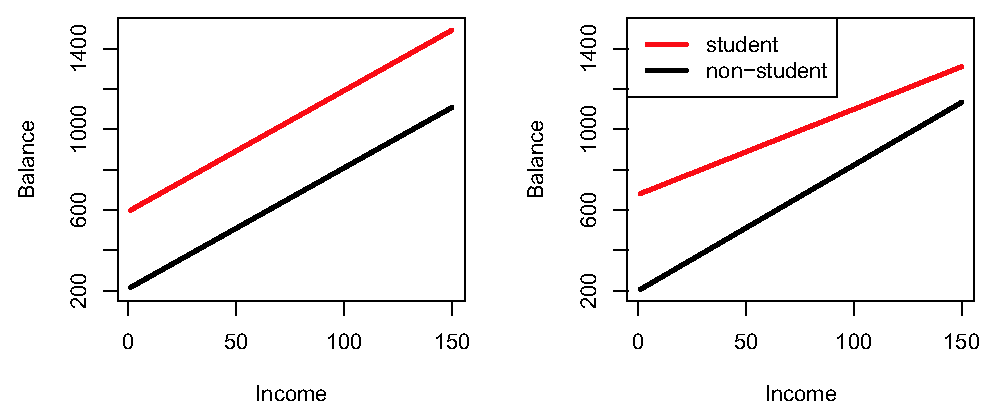
\includegraphics[scale=0.9]{images//3_7.eps}
\\~\\
\caption{Left: The model \eqref{non-interaction} with no interaction was fit, Right: The model \eqref{interaction} with interaction was fit }\label{figure-3.7}
\end{figure}

In the left panel of Figure \ref{figure-3.7}, we notice that Model \eqref{non-interaction} fit two parallel lines to the data, one for students and one for non-students.
The lines for students and non-students have different interceptions, $\beta_{0}+\beta_{2}$ versus $\beta_{0}$, but the same slope $\beta_{0}$. 
The fact that the lines are parallel means that according to Model \eqref{non-interaction}, the average effect on balance of a one-unit increase in income \underline{does not depend on whether or not the person is a student}. This assumption on the model is simply wrong, since in fact a change in income may have a very different effect on the credit card balance of a student versus a non-student. \\

This issue can be solved by adding an interaction variable into our model:
\begin{align}
y_{i} & \approx \beta_{0}+ \beta_{1} x_{i1} + \beta_{2} x_{i2} + \beta_{3} x_{i1} x_{i2}
\end{align}

\begin{itemize}
\item $x_{i1}$: Income for the ith person (Quantitative variable)
\item $x_{i2}$: whether the ith person is a student or not (Qualitative Dummy variable)
\item $x_{i1} x_{i2}$: Interaction term between Income($x_{i1}$) and Student($x_{i2}$)
\end{itemize}
The model with interaction term can be interpreted as below:
\begin{align}
{\rm balance}_{i} & \approx \beta_{0}+ \beta_{1} \times {\rm income}_{i} + \left\{
		\begin{array}{ll}
			\beta_{2}+ \beta_{3} \times {\rm income}_{i} , & \mbox{the ith person is a student}\\
			0, & \mbox{the ith person is not a student }\\
		\end{array} \right. \\
& = 	 \left\{
		\begin{array}{ll}
			(\beta_{0} + \beta_{2})+(\beta_{1} + \beta_{3}) \times {\rm income}_{i} , & \mbox{the ith person is a student}\\
			\beta_{0}+ \beta_{1} \times {\rm income}_{i}, & \mbox{the ith person is not a student }\\
		\end{array} \right.
\label{interaction}
\end{align}

In the right panel of Figure \ref{figure-3.7}, we notice that when we added a interaction term in our model, we get two different regression lines for the students and the non-students.
Those lines have different intercepts, $(\beta_{0}+\beta_{2})$ versus $\beta_{0}$ and different slopes, $(\beta_{1}+\beta_{3})$ versus $\beta_{1}$.
This allows for the possibility that changes in income may affect the credit card balances of students and non-students differently.


\subsubsection{\textbf{Potential problems for the assumptions of linear regression}}
\begin{enumerate}
\item Non-linearity of the response-predictors relationships
\item Correlation of error terms
\item Non-constant variance of error terms
\item Outliers
\item High leverage points
\item Collinearity 
\end{enumerate}

%=============================================================================================
\textbf{\color{blue}{1. Non-linearity of the Data}}:\\
Ideally, the residual plot will show no obvious pattern. 
The presence of a pattern may indicate a problem with non-linearity.

~\\~\\
How to detect Non-linearity:
\begin{itemize}
\item Plot the residuals($y_{i}-\hat{y}_{i}$) versus the fitted values $\hat{y}_{i}$ as a residual plot (Figure~\ref{figure-3.9})
\end{itemize}

How to solve Non-linearity:
\begin{itemize}
\item If the residual plot indicates non-linear in the data, then adding a non-linear transformations of the predictors, such as ${\rm log}X, \sqrt{X}, X^{2}$, in the regression model.
\end{itemize}

\begin{figure}[H]
\centering
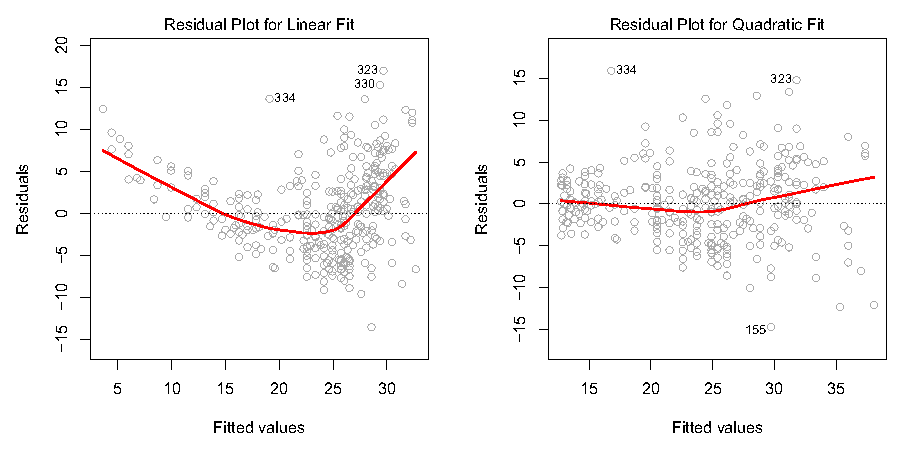
\includegraphics[scale=0.85]{images//3_9.eps}
\\~\\
\caption{Residual Plot, Left: a strong pattern in the residual indicates non-linearity if we fit our data to a linear model. Right: There is little pattern in the residual when we fit a quadratic model to the data}\label{figure-3.9}
\end{figure}

%=============================================================================================
\textbf{\color{blue}{2. Correlation of Error Terms}}:\\
In the assumption of the linear regression model, the error terms $\epsilon_{1}, \epsilon_{1}, \dots, \epsilon_{n}$ are uncorrelated. 
If in fact there is correlation among the error term, then \textbf{the estimated standard errors will tend to underestimate the true standard error}.
Such correlations frequently occur in time series data. In many cases, adjacent observations will have positive correlated errors.

How to detect Correlation of Error Terms:
\begin{itemize}
\item Plot the residuals($y_{i}-\hat{y}_{i}$) versus the observation (Figure~\ref{figure-3.10})
\item Identify obvious pattern in Figure~\ref{figure-3.10}
\end{itemize}

\begin{figure}[H]
\centering
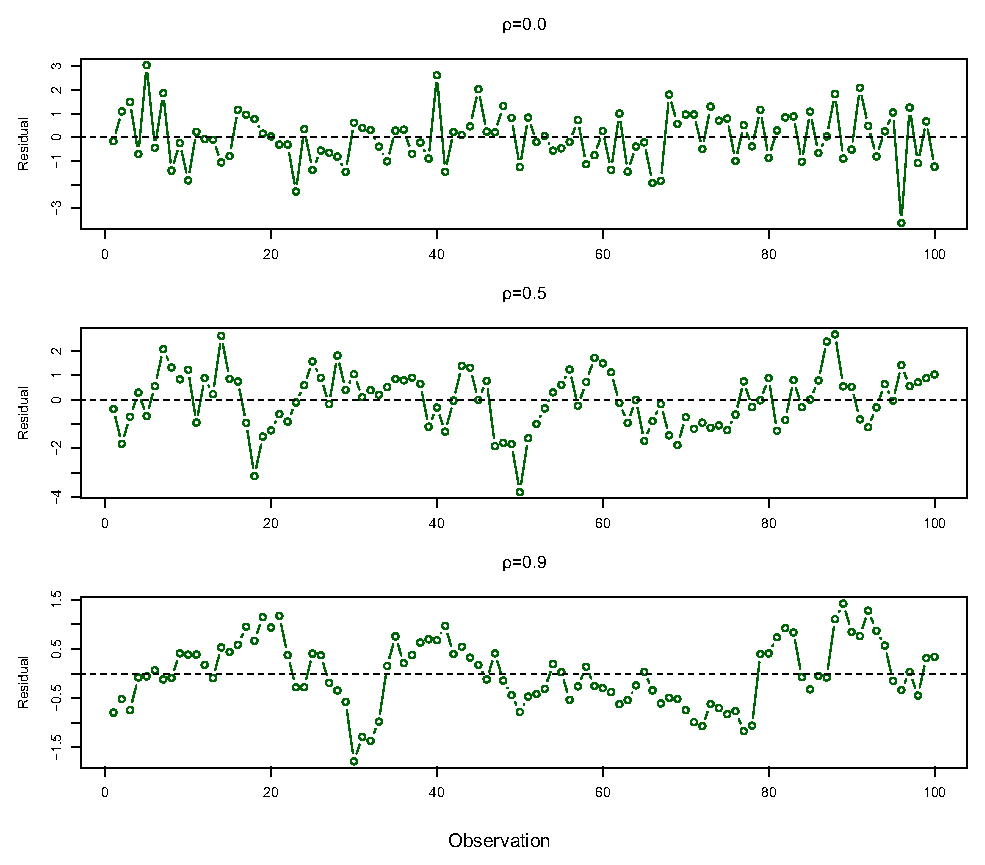
\includegraphics[scale=0.85]{images//3_10.eps}
\\~\\
\caption{Plots of residuals versus simulated time series observations with different levels of $\rho$}\label{figure-3.10}
\end{figure}

How to solve Correlation of Error Terms:
\begin{itemize}
\item If the residual plot indicates an obvious patten, then there might be a problem experiment design.
\end{itemize}

%=============================================================================================
\textbf{\color{blue}{3. Non-Constant Variance of Error Terms(Heteroscedasticity)}}:\\
In the assumption of the linear regression model, the variance of error terms are constant(${\rm Var}(\epsilon_{i})=\sigma^{2}$).
Unfortunately, it is often the case that the variances of the error terms are non-constant.

How to detect Non-Constant Variance of Error Terms:
\begin{itemize}
\item Plot residual plot to detect a funnel shape (Figure~\ref{figure-3.11})
\end{itemize}

\begin{figure}[H]
\centering
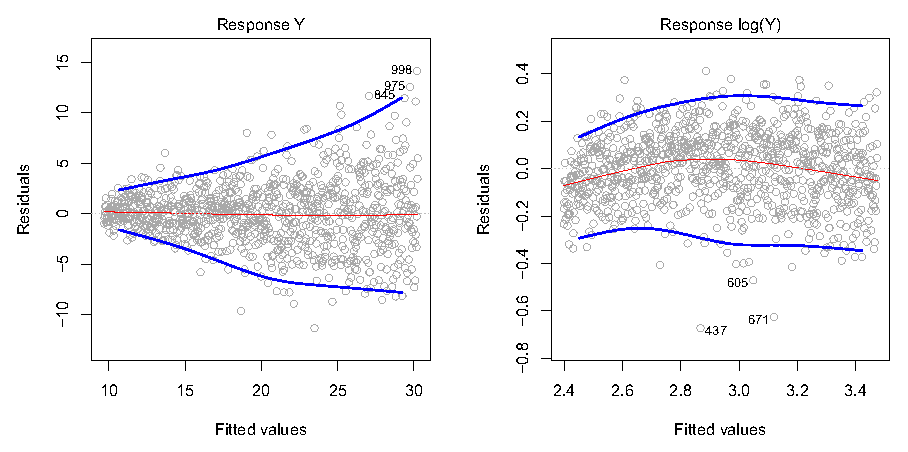
\includegraphics[scale=0.85]{images//3_11.eps}
\\~\\
\caption{}\label{figure-3.11}
\end{figure}

How to solve Non-Constant Variance of Error Terms:
\begin{itemize}
\item Transform the response $Y$ using a concave function such as ${\rm log}Y, \sqrt{Y}$
\item Or, fit our model by weighted least squares or generalized least squares
\end{itemize}

%=============================================================================================

\textbf{\color{blue}{4. Outliers}}:\\
How to detect Outliers:
\begin{itemize}
\item Plot residual plot and Studentized residual plot to detect outliers (Figure~\ref{figure-3.12})
\end{itemize}

\begin{figure}[H]
\centering
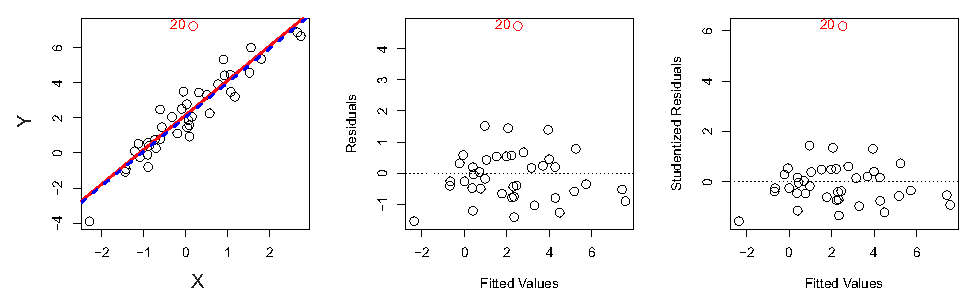
\includegraphics[scale=0.85]{images//3_12.eps}
\\~\\
\caption{}\label{figure-3.12}
\end{figure}

How to solve Outliers:
\begin{itemize}
\item Remove them
\end{itemize}
%=============================================================================================
\textbf{\color{blue}{5. High Leverage Points}}:\\
Leverage points means the observations have an unusual value of $x_{i}$. 
High leverage observations tend to have a sizable impact on the estimated regression model.

How to detect High Leverage Points:
\begin{itemize}
\item In order to identify an observation is a high leverage point, we compute the leverage statistic. 
A large value of this statistic indicates an observation with high leverage. (Figure~\ref{figure-3.13})
\end{itemize}
The leverage statistic for a simple linear regression where $y_{i} = \beta_{0} + \beta_{1}x_{i}$, ($p=1$, not including intercept)
\begin{gather}
h_{i} = \frac{1}{n} + \frac{(x_{i}-\bar{x})^{2}}{\sum\limits_{i'=1}^{n}(x_{i}-\bar{x})^{2}},{\rm where~} \frac{1}{n}<h_{i}<1
\end{gather}
For the average leverage $ \bar{h}= \frac{p}{n}$. So if a given observation has a leverage statistic that greatly exceeds $\frac{p+1}{n}$, then we suspect the corresponding point has high leverage ($x_{i}>\frac{p+1}{n} $). 
The proof of average leverage for a simple linear regression :

\begin{gather}
\bar{h} = \sum\limits_{i=1}^{n}\frac{h_{i}}{n} = \left(\sum\limits_{i=1}^{n} \frac{1}{n} + \sum\limits_{i=1}^{n} \frac{(x_{i}-\bar{x})^{2}}{\sum\limits_{i'=1}^{n}(x_{i}-\bar{x})^{2}}\right)/n = 2/n 
\end{gather}

\begin{figure}[H]
\centering
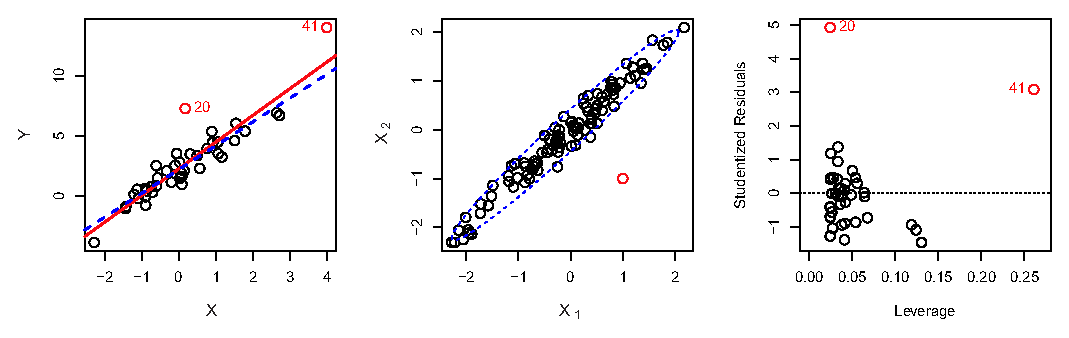
\includegraphics[scale=0.85]{images//3_13.eps}
\\~\\
\caption{}\label{figure-3.13}
\end{figure}

The leverage for multiple predictors:
\begin{align*}
\boldsymbol{\hat{\beta}} &= (\mathbf{X'}\mathbf{X})^{-1}\mathbf{X'}\mathbf{y} \\
\mathbf{\hat{y}}  &= \mathbf{X}\boldsymbol{\hat{\beta}}= \mathbf{X}(\mathbf{X'}\mathbf{X})^{-1}\mathbf{X'}\mathbf{y} \\
		&= \mathbf{H}\mathbf{y} \\
\mathbf{H} &= \mathbf{X}(\mathbf{X'}\mathbf{X})^{-1}\mathbf{X'} 
\end{align*}

The leverage, $h_{ii}$, quantifies the influence that the observed response $y_{i}$ has on its predicted value $\hat{y}_{i}$. 
That is, if $h_{ii}$ is small, then the observed response $y_{i}$ plays only a small role in the value of the predicted response $\hat{y}_{i}$. 
On the other hand, if $h_{ii}$ is large, then the observed response $y_{i}$ plays a large role in the value of the predicted response $\hat{y}_{i}$. 
It's for this reason that the $h_{ii}$ are called the "leverage".

Here are some important properties of the leverage:
\begin{itemize}
\item The leverage $h_{ii}$ is a measure of the distance between the $x_{i}$ value for the ith data point and the mean of the $x$ values for all $n$ data points.
\item The sum of the $h_{ii}$ equals $p+1$, the number of parameters (regression coefficients including the intercept).
\item The leverage $h_{ii}$ is a number between 0 and 1, inclusive.
\end{itemize}

\begin{framed}
\textbf{Example}\\

\begin{tabular}{lll}
Obs. & X  & Y   \\
\hline
1& 0.1& -0.0716\\
2& 0.45401& 4.1673\\
3& 1.09765& 6.5703\\
4& 1.27936& 13.815\\
5& 2.20611& 11.4501\\
6& 2.50064& 12.9554\\
7& 3.0403& 20.1575\\
8& 3.23583& 17.5633\\
9& 4.45308& 26.0317\\
10& 4.1699& 22.7573\\
11& 5.28474& 26.303\\
12& 5.59238& 30.6885\\
13& 5.92091& 33.9402\\
14& 6.66066& 30.9228\\
15& 6.79953& 34.11\\
16& 7.97943& 44.4536\\
17& 8.41536& 46.5022\\
18& 8.71607& 50.0568\\
19& 8.70156& 46.5475\\
20& 9.16463& 45.7762\\
21& 4& 40\\
\bottomrule
\end{tabular}


\textbf{R code:}
\footnotesize
\begin{lstlisting}[language=R]
x = matrix(c(0.1, 0.45401, 1.09765, 1.27936, 2.20611, 2.50064, 3.0403, 
3.23583, 4.45308, 4.1699, 5.28474,5.59238 ,5.92091,6.66066,6.79953,
7.97943,8.41536,8.71607,8.70156,9.16463, 4), ncol = 1)
x = matrix(cbind(rep(1,21),x), ncol=2)
H = x %*% solve(t(x)%*%x) %*% t(x)
H = round(H,4)
\end{lstlisting}
\end{framed}
%=============================================================================================
\textbf{\color{blue}{6. Collinearity}}:\\
Collinearity refers to the situation in which two or more predictor variables are closely related to one another. 
The importance of the predictor variables may be masked if we did not consider Collinearity. 

How to detect Collinearity:
\begin{itemize}
\item Compute correlation matrix for each predictor
\item Or, compute the variance inflation factor(VIF)
\end{itemize}

How to solve Collinearity:
\begin{itemize}
\item Drop one of the problematic variables from the regression model, since the other variable provides enough information.
\item Or, combine the collinear variables together to get a single predictor.
\end{itemize}

\section*{Reference}
\noindent
\begin{description}\itemsep=-2pt
\item {\MbQ\cH34}\z{\MiQ\cH16} (2012), {\MaQ\cH7}{\MbQ\cH84}\z{\MhQ\cH229}\z{\MeQ\cH78}\z{\McQ\cH228}\z{\MaQ\cH231}\z{\McQ\cH36}\z{\McQ\cH108}{\MaQ\cH8}, {\McQ\cH251}\z{\MhQ\cH23}, {\MkQ\cH49}\z{\MiQ\cH95}\z{\MaQ\cH199}\z{\MbQ\cH122}
\item Friedman, J., Hastie, T., \& Tibshirani, R. (2001). {\it{The elements of statistical learning}} (Vol. 1). Springer, Berlin: Springer series in statistics.
\item James, G., Witten, D., Hastie, T., \& Tibshirani, R. (2013). {\it{An introduction to statistical learning}} (Vol. 6). New York: springer.
\item Wasserman, L. (2013). {\it{All of statistics: a concise course in statistical inference}}. Springer Science \& Business Media.
\end{description}

\end{document}
